% Options for packages loaded elsewhere
\PassOptionsToPackage{unicode}{hyperref}
\PassOptionsToPackage{hyphens}{url}
%
\documentclass[
]{article}
\usepackage{amsmath,amssymb}
\usepackage{lmodern}
\usepackage{iftex}
\ifPDFTeX
  \usepackage[T1]{fontenc}
  \usepackage[utf8]{inputenc}
  \usepackage{textcomp} % provide euro and other symbols
\else % if luatex or xetex
  \usepackage{unicode-math}
  \defaultfontfeatures{Scale=MatchLowercase}
  \defaultfontfeatures[\rmfamily]{Ligatures=TeX,Scale=1}
  \setmainfont[]{Open Sans}
\fi
% Use upquote if available, for straight quotes in verbatim environments
\IfFileExists{upquote.sty}{\usepackage{upquote}}{}
\IfFileExists{microtype.sty}{% use microtype if available
  \usepackage[]{microtype}
  \UseMicrotypeSet[protrusion]{basicmath} % disable protrusion for tt fonts
}{}
\makeatletter
\@ifundefined{KOMAClassName}{% if non-KOMA class
  \IfFileExists{parskip.sty}{%
    \usepackage{parskip}
  }{% else
    \setlength{\parindent}{0pt}
    \setlength{\parskip}{6pt plus 2pt minus 1pt}}
}{% if KOMA class
  \KOMAoptions{parskip=half}}
\makeatother
\usepackage{xcolor}
\IfFileExists{xurl.sty}{\usepackage{xurl}}{} % add URL line breaks if available
\IfFileExists{bookmark.sty}{\usepackage{bookmark}}{\usepackage{hyperref}}
\hypersetup{
  pdftitle={Análisis habitacional},
  hidelinks,
  pdfcreator={LaTeX via pandoc}}
\urlstyle{same} % disable monospaced font for URLs
\usepackage[margin=1in]{geometry}
\usepackage{graphicx}
\makeatletter
\def\maxwidth{\ifdim\Gin@nat@width>\linewidth\linewidth\else\Gin@nat@width\fi}
\def\maxheight{\ifdim\Gin@nat@height>\textheight\textheight\else\Gin@nat@height\fi}
\makeatother
% Scale images if necessary, so that they will not overflow the page
% margins by default, and it is still possible to overwrite the defaults
% using explicit options in \includegraphics[width, height, ...]{}
\setkeys{Gin}{width=\maxwidth,height=\maxheight,keepaspectratio}
% Set default figure placement to htbp
\makeatletter
\def\fps@figure{htbp}
\makeatother
\setlength{\emergencystretch}{3em} % prevent overfull lines
\providecommand{\tightlist}{%
  \setlength{\itemsep}{0pt}\setlength{\parskip}{0pt}}
\setcounter{secnumdepth}{-\maxdimen} % remove section numbering
\usepackage{pdfpages}
\usepackage[default]{open sans}
\usepackage[T1]{fontenc}
\usepackage{graphicx}
\usepackage{fancyhdr}
\usepackage{hyperref}
\usepackage{xcolor}
\usepackage{sidecap}
\usepackage[spanish]{babel}
\pagestyle{fancy}
\renewcommand{\headrulewidth}{0pt}
\fancyhead{}
\setlength{\headheight}{23pt}
\lhead{
\includegraphics[width=7cm,height=140cm]{"./logos/logo_oecc.pdf"}}
\fancyfoot{}
\lfoot{
\includegraphics[width=5.0cm,height=140cm]{"./logos/muni.jpg"}}
\rfoot{\thepage}
\definecolor{graycustom}{HTML}{7b7b7e}
\usepackage{floatrow}
\floatsetup[figure]{capposition=top}
\renewcommand{\arraystretch}{1.5}
\usepackage{svg}
\usepackage{amsmath}
\usepackage{booktabs}
\usepackage{longtable}
\usepackage{array}
\usepackage{multirow}
\usepackage{wrapfig}
\usepackage{float}
\usepackage{colortbl}
\usepackage{pdflscape}
\usepackage{tabu}
\usepackage{threeparttable}
\usepackage{threeparttablex}
\usepackage[normalem]{ulem}
\usepackage{makecell}
\usepackage{xcolor}
\ifLuaTeX
  \usepackage{selnolig}  % disable illegal ligatures
\fi

\title{Análisis habitacional}
\author{}
\date{}

\usepackage[labelsep=endash]{caption} 

\AtBeginDocument{%
\renewcommand{\figurename}{Gráfico}
} 

\usepackage{floatrow}
\floatsetup[figure]{capposition=bottom} %ahí solucioné lo de la pos esto estaba en top

\fi
\setlength{\parindent}{14pt} %sangría


\begin{document}
%\begin{center}
%{\textbf{\Large Análisis habitacional de los hogares}}
%\end{center}
\hypertarget{ruxe9gimen-de-tenencia-habitacional-de-los-hogares}{%
\section{Régimen de tenencia habitacional de los
hogares}\label{ruxe9gimen-de-tenencia-habitacional-de-los-hogares}}

Para el análisis del régimen de tenencia habitacional de los hogares en
la Ciudad de Corrientes se utilizara como unidad de análisis al jefe/a de
hogar. Se elige esta unidad de análisis con el fin de disminuir las distorsiones que puede generar una posible correlación entre niveles de
hacinamiento y el régimen de tenencia de las viviendas de las personas.

\begin{table}[!h]

\caption{\label{tab:unnamed-chunk-7}Porcentaje de hogares en la Ciudad de Corrientes S/ régimen de tenencia habitacional}
\centering
\begin{tabular}[t]{lr}
\toprule
Régimen de tenencia & Porcentaje\\
\midrule
\cellcolor{gray!6}{Inquilino} & \cellcolor{gray!6}{21.18\%}\\
Irregular & 10.96\%\\
\cellcolor{gray!6}{Propietario} & \cellcolor{gray!6}{67.86\%}\\
\bottomrule
\end{tabular}
\end{table}

Como se puede ver en el cuadro \ref{tab:unnamed-chunk-7}, el 67.86\% de los hogares en la Ciudad
de Corrientes son propietarios de sus viviendas, mientras que el 32.14\%
se encuentran en situaciones de inquilinato u ocupación irregular.

\hypertarget{ruxe9gimen-de-tenencia-habitacional-seguxfan-el-guxe9nero-del-jefea-de-hogar}{%
\subsection{Régimen de tenencia habitacional según el género del jefe/a
de
hogar}\label{ruxe9gimen-de-tenencia-habitacional-seguxfan-el-guxe9nero-del-jefea-de-hogar}}

La jefatura de hogar de cada nucleo familiar puede estar a cargo de
hombres o mujeres. A continuación, se realiza el análisis del régimen de
tenencia según el género del jefe/a del hogar.

\begin{figure}[htbp!]
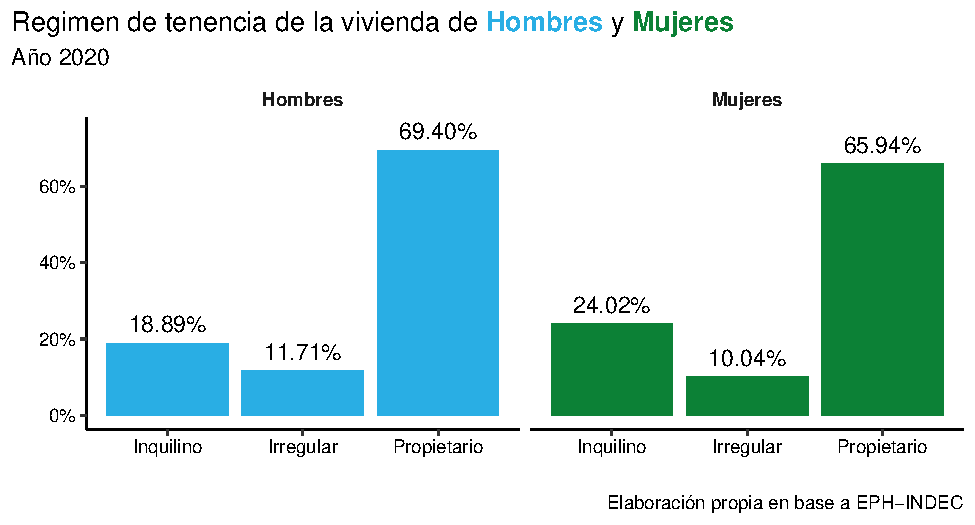
\includegraphics{habitacional_files/figure-latex/unnamed-chunk-8-1.pdf}
\caption{\label{fig:1}}
\end{figure}
\newpage
Como se puede ver en el gráfico \ref{fig:1}, las familias que tienen como jefa de
hogar a una mujer son mas propensas a no ser propietarias de su vivienda
y a encontrarse en condiciones de inquilinato que aquellas en las que el
jefe de hogar es un hombre.

\hypertarget{ruxe9gimen-de-tenencia-habitacional-seguxfan-la-edad-del-jefe-de-hogar}{%
\subsection{Régimen de tenencia habitacional según la edad del jefe de
hogar}\label{ruxe9gimen-de-tenencia-habitacional-seguxfan-la-edad-del-jefe-de-hogar}}

La edad del jefe de hogar puede condicionar el acceso a una vivienda
propia, siendo que la posibilidad de acumulación de ahorros es una
función del ingreso percibido a lo largo de la vida laboral.

A continuación se presenta el acceso a la vivienda para los distintos
rangos etarios.

\begin{figure}[htbp!]
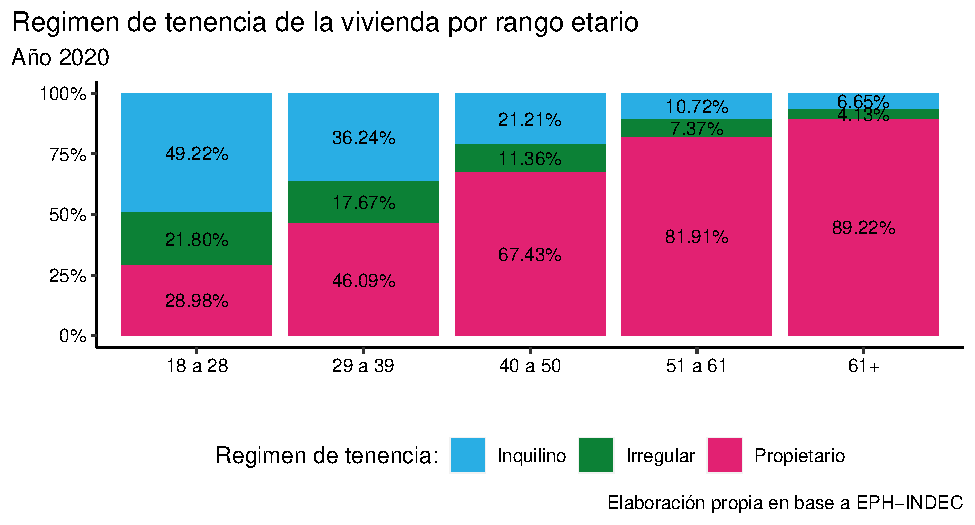
\includegraphics{habitacional_files/figure-latex/unnamed-chunk-9-1.pdf}
\caption{\label{fig:2}}
\end{figure}


En el Gráfico \ref{fig:2} se puede ver como la tenencia de una vivienda propia va
disminuyendo conforme es menor la edad de la persona que es jefe/a de
hogar. Para las familias con jefes/as de hogar jóvenes es mucho mas probable que se encuentren habitando una vivienda que es alquilada o que esta siendo ocupada de manera irregular.

\hypertarget{ruxe9gimen-de-tenencia-habitacional-seguxfan-la-incidencia-en-la-pobreza-del-jefe-de-hogar}{%
\subsection{Régimen de tenencia habitacional según la incidencia en la
pobreza del jefe de
hogar}\label{ruxe9gimen-de-tenencia-habitacional-seguxfan-la-incidencia-en-la-pobreza-del-jefe-de-hogar}}

La pobreza, especificamente la calculada a través del método de la linea
de la pobreza, intenta captar la incapacidad coyuntural de satisfacción
de las necesidades básicas de las familias. Estar por debajo de la linea
de la pobreza indica una situación de vulnerabilidad económica que puede
ser medida en un momento determinado. Sin embargo, la pobreza
estructural es considerablemente más nociva a nivel de marginación
social que la pobreza coyuntural. La falta de seguridad habitacional no
solamente se limita a la incapacidad temporal de satisfacer necesidades
básicas, sino que presenta un problema estructural de incapacidad en la
satisfacción de los derechos básicos de las personas.

Para analizar la seguridad habitacional de las personas pobres y no
pobres, medidas según el método de la linea de la pobreza, se presenta a
continuación el régimen de tenencia de las viviendas según la incidencia
en la pobreza del jefe/a de hogar.

\begin{figure}[htbp!]
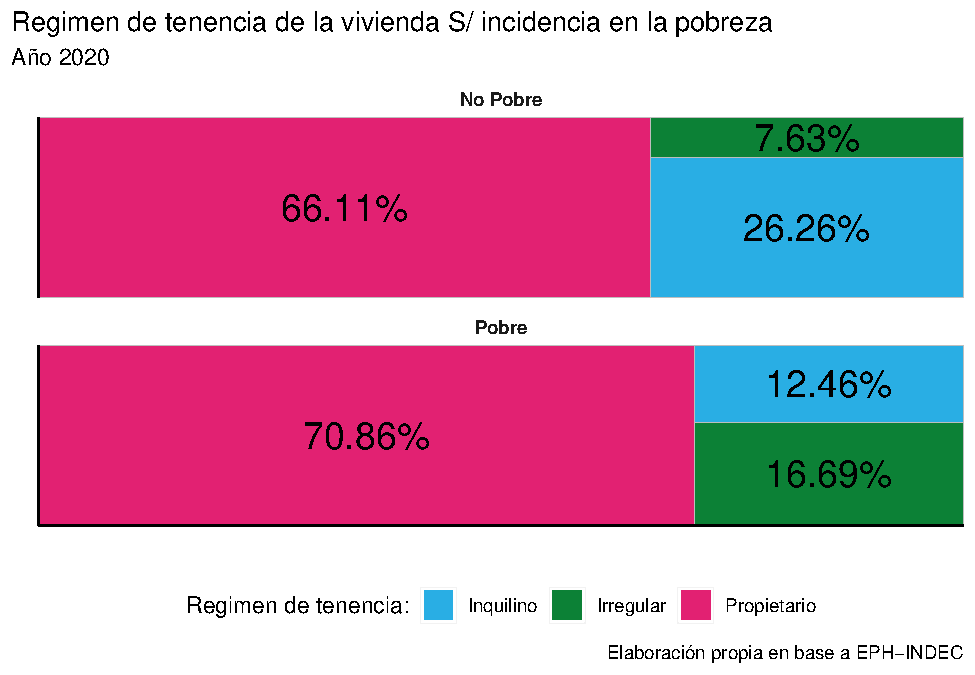
\includegraphics{habitacional_files/figure-latex/unnamed-chunk-10-1.pdf}
\caption{\label{fig:3}}
\end{figure}

En el gráfico \ref{fig:3} se puede ver una particularidad, la proporción de
propietarios de la vivienda en los casos que el jefe de hogar es pobre
es mayor que en el caso de los no pobres. Por otro lado, los pobres
tienen una mayor proporción de ocupación irregular que los no pobres, en
donde se incluyen casos como ocupación de viviendas, de terreno, etc.

\end{document}
